\documentclass[openany, 10pt]{article}
\usepackage[a4paper,margin=1in]{geometry} % Adjust margins as needed
\usepackage{enumitem}
\usepackage{listings}
\usepackage{hyperref}
\usepackage{tikz}
\usepackage{xcolor}

\usetikzlibrary{shapes.geometric, arrows, positioning, fit}

\lstdefinestyle{cpp-cuda-boxed}{
  language=C++,  % or CUDA ?
  basicstyle=\small\ttfamily,  % Tiny font size with monospace
  keywordstyle=\bfseries,  % Bold keywords
  stringstyle=\ttfamily,  % String in monospace
  numbers=none,  % No line numbers
  backgroundcolor=\color{white},  % White background
  frame=single,  % Box around the code
  rulecolor=\color{black},  % Box color (black)
  xleftmargin=10pt,  % Left margin
  xrightmargin=10pt,  % Right margin
  aboveskip=10pt,  % Space above the listing
  belowskip=10pt,  % Space below the listing
  showstringspaces=false,  % Don't show spaces in strings
  lineskip=-1pt,  % Adjust line height slightly to fit in tiny size
  morekeywords={__global__, __device__, __host__},  % Add CUDA specific keywords
  keepspaces=true,
}

\tikzstyle{startstop} = [rectangle, rounded corners, minimum width=3cm, minimum height=1cm,text centered, draw=black, fill=red!30]
\tikzstyle{process} = [rectangle, minimum width=3cm, minimum height=1cm, text centered, draw=black, fill=blue!30]
\tikzstyle{subprocess} = [rectangle, minimum width=3cm, minimum height=1cm, text centered, draw=black, fill=green!30]
\tikzstyle{arrow} = [thick,->,>=stealth]
\tikzstyle{stage} = [text centered, draw=black, dashed, inner sep=0.5cm]

\begin{document}
\begin{center}
    {\Huge \textbf{Project Proposal}} \\[2em]
\end{center}
\begin{flushright}
    \textbf{Tanzi Alessio} \\
    \textbf{Di Gregorio Antonino}
\end{flushright}
\section{Abstract}
Path tracing, a cornerstone algorithm in physically based rendering, provides realistic image synthesis by simulating the complex interactions of light. 
However, its computational demands make necessitate efficient implementations. This proposal explores a \textit{wavefront-based} approach to optimize the path tracing algorithm 
using NVIDIA's CUDA framework, leveraging GPU parallelism to maximize throughput and minimize latency. \par
Unlike traditional monolithic kernel implementations, the wavefront approach decomposes path tracing into distinct stages, such as ray generation, 
intersection testing, shading, and path termination. \par 
Each stage operates as an independent kernel, allowing for reduced divergence across threads. It is possible to combine such a pipeline structure with the concept of 
\textit{packet tracing}, meaning processing multiple spatially coherent rays in parallel. The project aims to exploit CUDA's features, such as shared memory, and streams, 
to efficiently manage these wavefront stages while addressing synchronization challenges inherent in multi-kernel workflows. \par
By implementing and benchmarking this wavefront path tracing system, the project seeks to explore the aforementioned implementation and measure it terms of render time to 
reach a given variance, and comparing these to exising rendering systems like \textit{PBRT-v4} and \textit{MoonRay}.\par
% Inserire gli ultimi avanzi per l'algoritmo di path tracing, quindi rendering spettrale, quindi geatione bidirezionale della luce, 
% quindi metropolis hastings
Our GPU implementation will use \href{https://raytracing-docs.nvidia.com/optix8/guide/index.html}{NVIDIA OptiX}, while our CPU based implementation will use
\href{https://github.com/RenderKit/embree}{Embree}
\section{Theory Overview}
The algorithm starts by defining a \textit{Camera Model}, whose main purpose is to 
\begin{itemize}[topsep=0pt, noitemsep] 
  \item generate Camera Rays 
  \item set a given sample time
  \item culling out of view objects based on render distance and field of view
  \item computing depth of field - related blur by using the gaussian lens model. Implemented by samplng a point on the circular lens and 
    shooting 2 rays instead of one. The former going through the certer of the lens and the latter going through the sampled point, and then
    averaging the two computed radiance contribution
\end{itemize}
Once a camera has generated and propagated them through the scene, such rays will carry radiance over the inverse path they have defined.\par
When such process has terminated, we end up with a grid of radiance sample points on the image plane (which we will refer to as "film").\par
Once we computed a radiance grid, a \textit{Sensor Model} computes a tristimulus response by storing three RGB matching functions, which are SPDs. They compute 
a response from the incident radiance distribution coming from a sampled point while applying \textit{White Balancing} through the von Kries Transform.\par
This lasat step will give us a grid of irradiance responses, which now have to be aggregated following the grid of actual pixels, superimposed on our grid of 
adiemnsional samples. Instead of a common average of all samples falling under a pixel, we use a weighted average proportional to the probability of sampling the given 
sample position on the film (\textit{weighted importance Monte Carlo Estimator}).\par
Determining how many and where the samples should be placed on the film before the rendering process starts is determined by a \textit{Sampler}, which can follow the Halton 
smpling formula.\par
Image reconstruction from the set of irradiance response samples from the Sensor instead needs a \textit{Reconstruction Filter} application. which can be eg a Box filter, or 
a more sophisticated one like Mitchell-Netravali's filter, which exhalts the edges.\par
Since we analysed the beginning and end of the process, we briefly turn to what happens during ray propagation. Such a ray travels through a medium, hence its traveling radiance
should be multiplied by a Transmission coefficient\footnote{accounting for phenomena such as absorption and scattering} determined 
by Beer's Law and implemented by defining surfaces represenging mediume volume boundaries, but we'll ignore it 
and instead assume the ray travels through void space, hence transporting radiance in a lossless fashion.\par
Therefore we focus to 
\begin{itemize}[topsep=0pt, noitemsep]
  \item Ray Interction algorithms
  \item Surface Reflection models as BRDFs or BTDFs (probability distributions of incoming direction + reflected radiance computation)
\end{itemize}
Starting from the first bullet point: Each surface, whether represented by a triangular mesh, bezier patches, ..., should be aggregated in a 
\textit{Spatial Structure}\footnote{Which also allow for instancing to be better implemented},
such as a \textit{Bounding Volume Hierarchy}\footnote{stored in a linearized layout using Morton Encoding}, which partitions the scene into nodes, whose splitting 
can be applied with a criteria such as Hierarchical lienar bounding volume hierarchy by using corton-curve based clustering of nodes.\par
Once a BVH of the scene has been built, its intersection test is handled by a recursive call to a function checking whether the ray crosses a given box or not, and if yes,
visits all children nodes, until we hit a leaf bounding box. Once we reach such condition, primitive-specific intersection tests can be fired, and all other pending BVH 
intersection tests stopped.\par
Once a surface intersection has been found, its \textit{Reflection Model} comes into play.\par Such model can be represented in a variety of ways, such as Measured data 
carefully sampled on the unit sphere of directions and then reconstructed, or mathematical parametrized model. A widely popular example of the latter category are the family of
BSDFs using \textit{Microfacet Theory}, meaning modeling a surface's optical properties as being composed by many minuscule planes, all of them obeying to Reflection law and 
snell's Law to compute trasmitted and reflected directon, and Fresnel's Equations to compute radiance transmittance and reflectance factors.\par
In particular, microfacet models define a normal distribution function, to sintesize the orientation of the infinitely many facets composing the geometry, from which, by 
introducing factors accounting for phenomena such as shadowning and masking of light rays, a formulation of a BRDF such as the Torrance-Sparrow model can be formulated. Summary
\begin{itemize}[topsep=0pt, noitemsep]
  \item From an NDF we can sample a incoming direction
  \item From the BSDF Torrance-Sparrow model we can compute the Reflectance/Transmittance factor, which combines the Fresnel's Equations with geometry contributions
\end{itemize}
Such equations make use of parameters such as base color, roughness, metallic, ie optical characteristics of the material, which can be defined either as a single color or
can be encoded into a \textit{Texture}. Such textures handling requires the following procedures
\begin{itemize}[topsep=0pt, noitemsep]
  \item Texture Source: Constant, Image, Mathematical Function
  \item Texture Coordinate Generation Function: Typically performed through UV Mapping
  \item Texture Sampling an Antialiasing: Texture functions are also sampled, hence all frequencies beyond the Nyquist Limit must be removed with box filtering. To do so, we
    need to know which portion of the texture a pixel area centered in the camera sample sees. Such information can be tracked by implementing the so called 
    \textit{Ray Differentials}, meaning that, for each camera ray, two additional rays are shot (only for the first intersection), displaced one pixel in the x axis and anotehr 
    displaced in the y axis
\end{itemize}
Texture Sources of type Image present a further complication, as they are 2D arrays of point sampled values themselves. This means that the area defined by the ray differential
in uv space may encompass a given number of texels (minification) or be contained in a fraction of one or more texels (magnification). Such a problem is fixed by introducing
\textit{MipMapping}, 
% pagina 668. Cosa succede nei rimbalzi successivi dove non hai ray differentials? Campioni normalmente con mipmapping forse
which involves creating multiple subsampled versions of the image, and choosing at evaluation time the mip level which makes it so that the filter area defined by the sampling
procedure covers 4 texels. From the 3 points defined by the ray differential, we can define either a box filter or an elliptical one (EWA). The result from this filtering
procedure will be a sample from an image texture.\par
\section{Brief of the Algorithm}
\begin{figure}[t]
  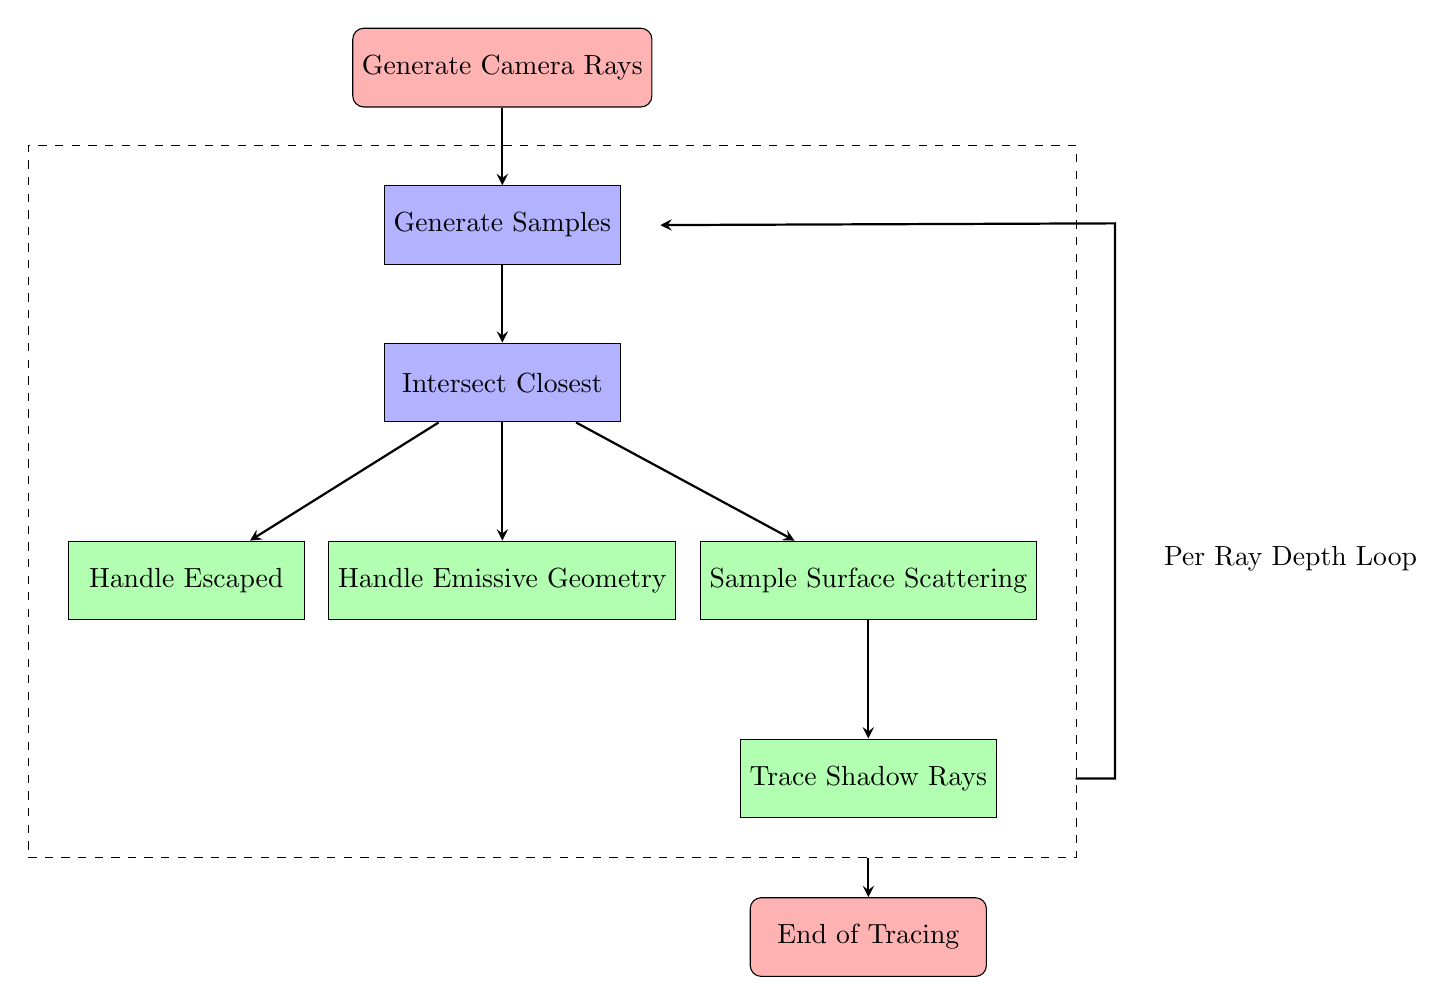
\begin{tikzpicture}[node distance=1.5cm]
  % Nodes for main flow
  \node (start) [startstop] {Generate Camera Rays};
  \node (generate) [process, below of=start, yshift=-0.5cm] {Generate Samples};
  \node (intersect) [process, below of=generate, yshift=-0.5cm] {Intersect Closest};

  % Sub-process nodes for Intersect Closest
  \node (escaped) [subprocess, below left=1.5cm and 1cm of intersect] {Handle Escaped};
  \node (emissive) [subprocess, below=1.5cm of intersect] {Handle Emissive Geometry};
  \node (scattering) [subprocess, below right=1.5cm and 1cm of intersect] {Sample Surface Scattering};

  % Sub-process for Sample Surface Scattering
  \node (shadow) [subprocess, below=1.5cm of scattering] {Trace Shadow Rays};

  % Loops for depth
  \node (loopstart) [stage, fit={(generate) (shadow) (intersect) (escaped) (emissive) (scattering)}] {};

  % Loops for depth (right label)
  \node (looplabel) [above right=2.0cm and 2.0cm of shadow] {Per Ray Depth Loop};

  % End
  \node (end) [startstop, below=1cm of shadow] {End of Tracing};

  % Arrows for main flow
  \draw [arrow] (start) -- (generate);
  \draw [arrow] (generate) -- (intersect);

  % Arrows to sub-processes
  \draw [arrow] (intersect) -- (escaped);
  \draw [arrow] (intersect) -- (emissive);
  \draw [arrow] (intersect) -- (scattering);

  \draw [arrow] (scattering) -- (shadow);

  % Loop back to start of depth
  \draw [arrow] (shadow.east) ++(1,0) -- ++(0.5,0) -- ++(0, 7.05) -- ([xshift=0.5cm]generate.east);

  % Arrow to end
  \draw [arrow] (shadow.south) ++(0,-0.5) -- ++(0,-0.3) -- (end.north);

  \end{tikzpicture}
  \caption{Diagram showing kernel execution for a GPU path tracer with the wavefront architecture}
  \label{gif}
\end{figure}
While in a typical CPU implementation, introducing multiprocessing is done through decomposition of the image in tiles and let each core process a packet of rays generated 
inside each with the use of SIMD instruction, such an approach in the GPU is fundamentally flawed by the fact that there aren't nearly enough tiles in a typical high resolution
image to prepare enough workloads to achieve a sufficient GPU hardware utilization. Hence there are fundamentally two approaches to a GPU Path tracer, detailed below:
% labelwidth area riservata a labels, labelsep separazione tralabel e testo, leftmargin il margine
\begin{itemize}[topsep=0pt, noitemsep, labelwidth=3cm, labelsep=1em, leftmargin=4cm] 
  \item[\textbf{megakernel}] assign each pixel sample to a thread, and execute a kernel which handles the whole path tracing algorithm. Since Rays will hit different spatial 
    positions, it is reasonable that the major problem for this approach is \texttt{Divergence}, which can be mitigated by organizing Queues of coherent work units, executed by 
    each warp. Even with this, the other disadvantage of such approach is that the code amout of the kernel is huge. Furthermore, even with job scheduling, it is impossible to 
    completely eliminate divergence
  \item[\textbf{wavefront}] Separate the main operations into different kernels. This allows to allocate less registers to simpler kernels and to handle the complexity and 
    convergence problems which arise from the megakernel approach. Nevertheless, they pay the price for such additional flexibility in memory traffic, since the only way kernels
    have to communicate is through Global Memory\footnote{we are assuming rendering over a single GPU}
\end{itemize}
We will follow the latter approach, hence having
\begin{itemize}[topsep=0pt, noitemsep]
  \item A first kernel generating camera samples and keeping them in device memory for later use
  \item find closest interaction and store intersection information in 3 different queues, one for escaped rays, one for rays that hit a light, and one for
    rays that hit a surface
  \item the kernels of escaped rays and of rays which hit an emissive geometry are responsible to update radiance estimation over the path traced by therr rays 
  \item the kernels which handle each type of surface are responsible to compute transmittance and reflectance factors, and enqueue indirect rays and shadow rays respectively
    for the shadow rays step and the next iteration
  \item most of the kernels, as mentioned above, generate some indirect rays which need to be traced again, therefore the specified kernels are launched again a number of times
    specified by the maximum depth (or bounces) for the algorithm, as shown in Figure \ref{gif}
\end{itemize}
Final Notes:
\begin{itemize}[topsep=0pt, noitemsep]
  \item Emphasis is drawn to the memory layout of each of the object (eg. surface interaction information, ray data), which in typical implementation are 
    stored in a Structure of Arrays layout
  \item The scenes will be stored in the \texttt{.pbrt} format, for which scenes are already available in this \href{https://github.com/mmp/pbrt-v4-scenes}{GitHub Link},
    and a parser is available on the \href{https://github.com/mmp/pbrt-v4}{PBRT-v4 Repository}
  \item The loop for kernel execution is made on the CPU over \textit{Wavefront Depth}. One possible approach is to ignore the state of execution of the algorithm, meaning 
    that the CPU will still launch the kernels up to max depth, even if all rays escape the scene after the first intersection test
\end{itemize}
\section{Minimal Outline Code Examples}
CPU code
\begin{lstlisting}[style=cpp-cuda-boxed]
#include <embree3/rtcore.h>
#include <iostream>
#include <cmath>
#include <vector>

// Helper: Vec3 class
struct Vec3 {
    float x, y, z;
    Vec3(float x = 0, float y = 0, float z = 0) : x(x), y(y), z(z) {}
    Vec3 operator+(const Vec3 &v) const { return {x + v.x, y + v.y, z + v.z}; }
    Vec3 operator-(const Vec3 &v) const { return {x - v.x, y - v.y, z - v.z}; }
    Vec3 operator*(float s) const { return {x * s, y * s, z * s}; }
    Vec3 normalize() const {
        float len = std::sqrt(x * x + y * y + z * z);
        return {x / len, y / len, z / len};
    }
};

// Ray-triangle intersection kernel
bool traceRay(RTCScene scene, const Vec3 &origin, const Vec3 &dir, Vec3 &hit) {
    RTCIntersectContext context;
    rtcInitIntersectContext(&context);

    RTCRayHit rayHit;
    rayHit.ray.org_x = origin.x;
    rayHit.ray.org_y = origin.y;
    rayHit.ray.org_z = origin.z;
    rayHit.ray.dir_x = dir.x;
    rayHit.ray.dir_y = dir.y;
    rayHit.ray.dir_z = dir.z;
    rayHit.ray.tnear = 0.001f;
    rayHit.ray.tfar = std::numeric_limits<float>::infinity();
    rayHit.hit.geomID = RTC_INVALID_GEOMETRY_ID;

    rtcIntersect1(scene, &context, &rayHit);

    if (rayHit.hit.geomID != RTC_INVALID_GEOMETRY_ID) {
        hit = origin + dir * rayHit.ray.tfar; // Compute hit point
        return true;
    }
    return false;
}

int main() {
    RTCDevice device = rtcNewDevice(nullptr);
    RTCScene scene = rtcNewScene(device);

    // Add triangle geometry (minimal example)
    RTCGeometry geom = rtcNewGeometry(device, RTC_GEOMETRY_TYPE_TRIANGLE);
    Vec3 vertices[] = {{0, 0, 0}, {1, 0, 0}, {0, 1, 0}};
    unsigned int indices[] = {0, 1, 2};
    rtcSetGeometryVertexAttributeCount(geom, 1);
    rtcSetSharedGeometryBuffer(geom, RTC_BUFFER_TYPE_VERTEX, 0, 
                               RTC_FORMAT_FLOAT3, vertices, 0, sizeof(Vec3), 3);
    rtcSetSharedGeometryBuffer(geom, RTC_BUFFER_TYPE_INDEX, 0, RTC_FORMAT_UINT3,
                                indices, 0, sizeof(unsigned int[3]), 1);
    rtcCommitGeometry(geom);
    rtcAttachGeometry(scene, geom);
    rtcReleaseGeometry(geom);
    rtcCommitScene(scene);

    // Minimal ray tracing loop
    Vec3 origin(0.5, 0.5, -1), dir(0, 0, 1), hit;
    if (traceRay(scene, origin, dir, hit))
        std::cout << "Hit at: " << hit.x << ", " << hit.y << ", " 
                  << hit.z << "\n";
    else
        std::cout << "No hit\n";

    rtcReleaseScene(scene);
    rtcReleaseDevice(device);
    return 0;
}

\end{lstlisting}
GPU code
\begin{lstlisting}[style=cpp-cuda-boxed]
#include <optix.h>
#include <optix_stubs.h>
#include <cuda_runtime.h>
#include <iostream>

// OptiX pipeline and program group handles
OptixDeviceContext context;
OptixPipeline pipeline;
OptixProgramGroup raygen_prog, miss_prog, hit_prog;

// CUDA device code: Raygen program
extern "C" __global__ void __raygen__main() {
    const uint3 idx = optixGetLaunchIndex();
    const float3 origin = make_float3(0.5f, 0.5f, -1.0f);
    const float3 dir = make_float3(0.0f, 0.0f, 1.0f);

    // Trace the ray
    unsigned int payload = 0;
    optixTrace(optixLaunchParams.traversable, origin, dir,
               0.001f, 1e16f, 0.0f, OptixVisibilityMask(255),
               OPTIX_RAY_FLAG_NONE, 0, 1, 0, payload);

    // Write output (dummy result)
    optixLaunchParams.image[idx.y * optixLaunchParams.width + idx.x] = payload;
}

// Host code
int main() {
    // Initialize OptiX context
    CUcontext cu_ctx = 0;
    cuInit(0);
    OptixDeviceContextOptions options = {};
    optixDeviceContextCreate(cu_ctx, &options, &context);

    // Set up pipeline, program groups, and modules (not shown for brevity)
    // ...

    // Launch kernel
    CUdeviceptr d_output;
    cudaMalloc(&d_output, width * height * sizeof(unsigned int));

    OptixLaunchParams params = {};
    params.image = reinterpret_cast<unsigned int*>(d_output);
    params.width = width;
    params.height = height;

    optixLaunch(pipeline, 0, d_output, sizeof(OptixLaunchParams), 
                &params, width, height, 1);
    cudaDeviceSynchronize();

    // Cleanup (release pipeline, context, etc.)
    optixPipelineDestroy(pipeline);
    optixDeviceContextDestroy(context);

    return 0;
}
\end{lstlisting}
% inserire le due fondamentali famiglie di architetture, cioe il megakernel e wavefront. andremo con il wavefront, un po perche 
% e quello che segue PBRT e un po perche e quello che implementano in hardware i RT cores delle GPU moderne
% 
% Useremo compute capability cc6.0 perche ho una gtx 1070, quindi no thread independent scheduling, no cooperative groups.
% Dire cosa deve fare ogni kernel e che tipo di sincronizzazione ci deve essere, quindi se si utilizzamo le streams o i graphs, 
% se lo possiamo fare lo schema si presta bene con i grafi
% dettagliare il memory layout e quindi come gestire la shared memory
% 
% embree -> CPU ray tracing
% optiX  -> GPU ray tracing

% double buffering per streammare tutti i risultati alla cpu per evalugtare la varianza
\end{document}
